% EN48 c09 | 原书 p.114–130（PDF 123–139） | 第 5 章 §5.1–5.2
% 骨架文件：标题行已设定，正文由译者填写。每页起首用 % ===== 原书 p.N ===== 注释标记。
\section{主定理}

\subsection{HMS 计算}

% ===== 原书 p.114 =====
\begin{remark}\label{rem:tqft}
在物理中，函子 $(Y,v_0)\mapsto H^0(\mathrm{FS}(Y,v_0))$ 可称为\emph{拓扑量子场论}（topological quantum field theory），简称 TQFT。也就是说，TQFT 的第一部分是从某些流形到向量空间的函子。更多背景可见 Segal 的讲义 [Seg]。本文考虑的是 Donaldson--Fukaya 范畴，完整的 $A_\infty$-范畴等价是未来的方向。要过渡到 $H^0$，我们需要知道微分。
\end{remark}

\begin{remark}\label{rem:diff}
回忆上文给出的 Fukaya--Seidel 范畴的定义。然而，要在上同调层面证明全忠实的 HMS 嵌入，我们需要计算 $\mathrm{FS}(Y,v_0)$ 上的微分，以求出 $H^0(\mathrm{FS}(Y,v_0))$ 中的态射群；仅知道微分存在还不够。此外，上文的定义使用正则 $J$，排除了球泡（sphere bubbling）；这一结论来自对 McDuff--Salamon 结果的改造。其哲学是：假设「一般的 $J$」对应「一般相交」中的一般性，则 0 维球族中所有点之并为两点，1 维圆盘族中所有点之并为三点；因此在 6 维流形中，二者一般不相交。
\end{remark}

然而，下文计算微分时我们使用标准 $J_0$，即环面坐标中乘以 $i$ 的复结构。此时无法排除球泡。原因在于 $H_2(v_0^{-1}(0))$ 非平凡：$v_0^{-1}(0)$ 是 $Y$ 的中心纤维，它来自 $J_0$-复子流形，因为 $v_0$ 关于 $J_0$ 全纯。非零的 Dolbeault 上同调说明这些球不正则；具体说，由 Riemann--Roch，$\bar\partial$ 算子的余核正是 Dolbeault 上同调。我们用 Gromov--Witten 不变量理论描述 [KL19] 中给出的球计算；再用 polyfold 理论对 $\bar\partial_J$ 作抽象扰动 [BFW17]，说明非正则 $J$ 下 Fukaya 范畴不变。于是 polyfold 给出的 Fukaya 范畴，与直接用 $J_0$ 算出的范畴拟同构。

\transnote{这里的要害是：正则性只对「一般的 $J$」成立，而 $J_0$ 是特殊的复结构。$J_0$ 下出现的全纯球并不正则，因此不能把它们当作 $J$-全纯曲线来数；作者改用 polyfold 的抽象扰动绕开这一点。阅读下文时，凡出现 $J_0$ 的计算，都应理解为「先对 $J$ 计数，再取极限」。}

% ===== 原书 p.115 =====
于是，用 $J_0$ 直接计算微分，即可把 HMS 两边的范畴对应起来。

\begin{remark}[记号]\label{rem:notation-M}
大写 $M^k$ 表示 $Y$ 全空间上的结构映射；小写 $M^k$ 表示环面纤维上的结构映射。
\end{remark}

\begin{lemma}\label{lem:compute-d}
$\partial:CF(\ell_{i+1},\ell_j)[-1]\to CF(\ell_i,\ell_j)$ 可由全体 $z$ 的 $\partial:CF(t_z,\ell_i)\to CF(t_z,\ell_i)$ 数据算出。
\end{lemma}

\begin{proof}
设 $p_j$ 为 $\ell_j$ 与 $t_z$ 的交点；设 $t^k_{i,j}$ 为 $\ell_i\cap\ell_j$ 的第 $k$ 个交点，其中 $0\le k<(i-j)^2$，如上面 Fukaya--Seidel 范畴定义所述。下图的第一与最末竖直箭头可以算出，我们要算中间的箭头。设微分把 $p_j$ 送到 $C(z)\cdot p_j$；这里 $C(z)$（count）是一个待计算的计数，它依赖 $z$ 而不依赖 $j$。这个图让我们求出中间的竖直箭头。注意：大写指沿底空间中的曲线平行移动小写纤维拉格朗日。论证的关键是 Leibniz 法则。见图 5.1。
\[
\begin{tikzcd}[column sep=2.8em, row sep=3.4em]
\hom(\ell_j,t_z)\otimes\hom(\ell_{i+1},\ell_j)\ni p_j\otimes t^k_{i+1,j}
  \arrow[r,"M^2"] \arrow[d,"\partial"'] &
\hom(\ell_{i+1},t_z)\ni M^2(p_j,t^k_{i+1,j}) \arrow[d,"\partial"] \\
\hom(\ell_j,t_z)\otimes\hom(\ell_i,\ell_j)\ni C p_j\otimes\partial(t^k_{i+1,j})
  \arrow[r,"M^2"'] &
\hom(\ell_{i+1},t_z)\ni \partial(M^2(p_j,t^k_{i+1,j}))
\end{tikzcd}
\]

特别地，由乘积求导的 Leibniz 法则，有
\[
M^1(M^2(p_j,t^k_{i+1,j}))
=M^2(M^1(t^k_{i+1,j}),p_j)+M^2(t^k_{i+1,j},M^1(p_j))
=M^2(M^1(t^k_{i+1,j}),p_j),
\]
因为 $M^1(p_j)=0$：$p_j$ 的次数为 0，而两拉格朗日的其他交点处没有 1 次元；注意 $p_i$ 的次数为 $-1$。注意 $M^1(t^k_{i+1,j})$ 正是我们要求的对象。又因在米色区域纤维丛平凡，可在纤维中数以 $p_i,p_j,t^k_{i+1,j}$ 为顶点的三角形，得 $M^2(p_j,t^k_{i+1,j})=D(z)\cdot p_i$，其中 $D(z)$ 是某个函数。再由同伦论证算得 $M^1(p_i)=C(z)\cdot p_j$。于是上式给出
\[
C(z)\cdot D(z)\cdot p_j=M^2(M^1(t^k_{i+1,j}),p_j),
\]
由此可算出 $M^1(t^k_{i+1,j})$。
\end{proof}

\transnote{图中两行并不是两个独立命题：上排是「按定义」的一侧，下排是「按计算」的一侧。竖直箭头 $\partial$ 把上排元素送到下排，横向的 $M^2$ 是乘积。作者先算出首末两条竖直箭头，再用交换性反求中间一条。读图时注意 $M^2$ 的两个自变量顺序：在 $M^2(p_j,t^k_{i+1,j})$ 中 $p_j$ 在前。}

\transnote{$M^1(p_j)=0$ 的理由是次数：$p_j$ 是 0 次交点，而同处没有 1 次交点，故微分的 0 次分量作用在 $p_j$ 上为零。相对地，$p_i$ 的次数为 $-1$，所以 $M^1(p_i)$ 不必为零。这一处最易把 $p_i$ 与 $p_j$ 的次数记反。}

我们愿意用 $t_z$ 而不用某个 $\ell_j$，是因为这样可以数边界落在矩映射原像中的圆盘，如 [CO06]。把 $t_z$ 沿 U 形曲线平行移动得到的拉格朗日 $T_z$，对应镜像侧点 $z$ 处的赋值截面。因此，一旦知道全体 $t_z$ 的态射群，就知道了任意 $\ell_i$ 与 $\ell_j$ 之间的 hom。

% ===== 原书 p.116 =====
\begin{figure}[!htbp]
\centering
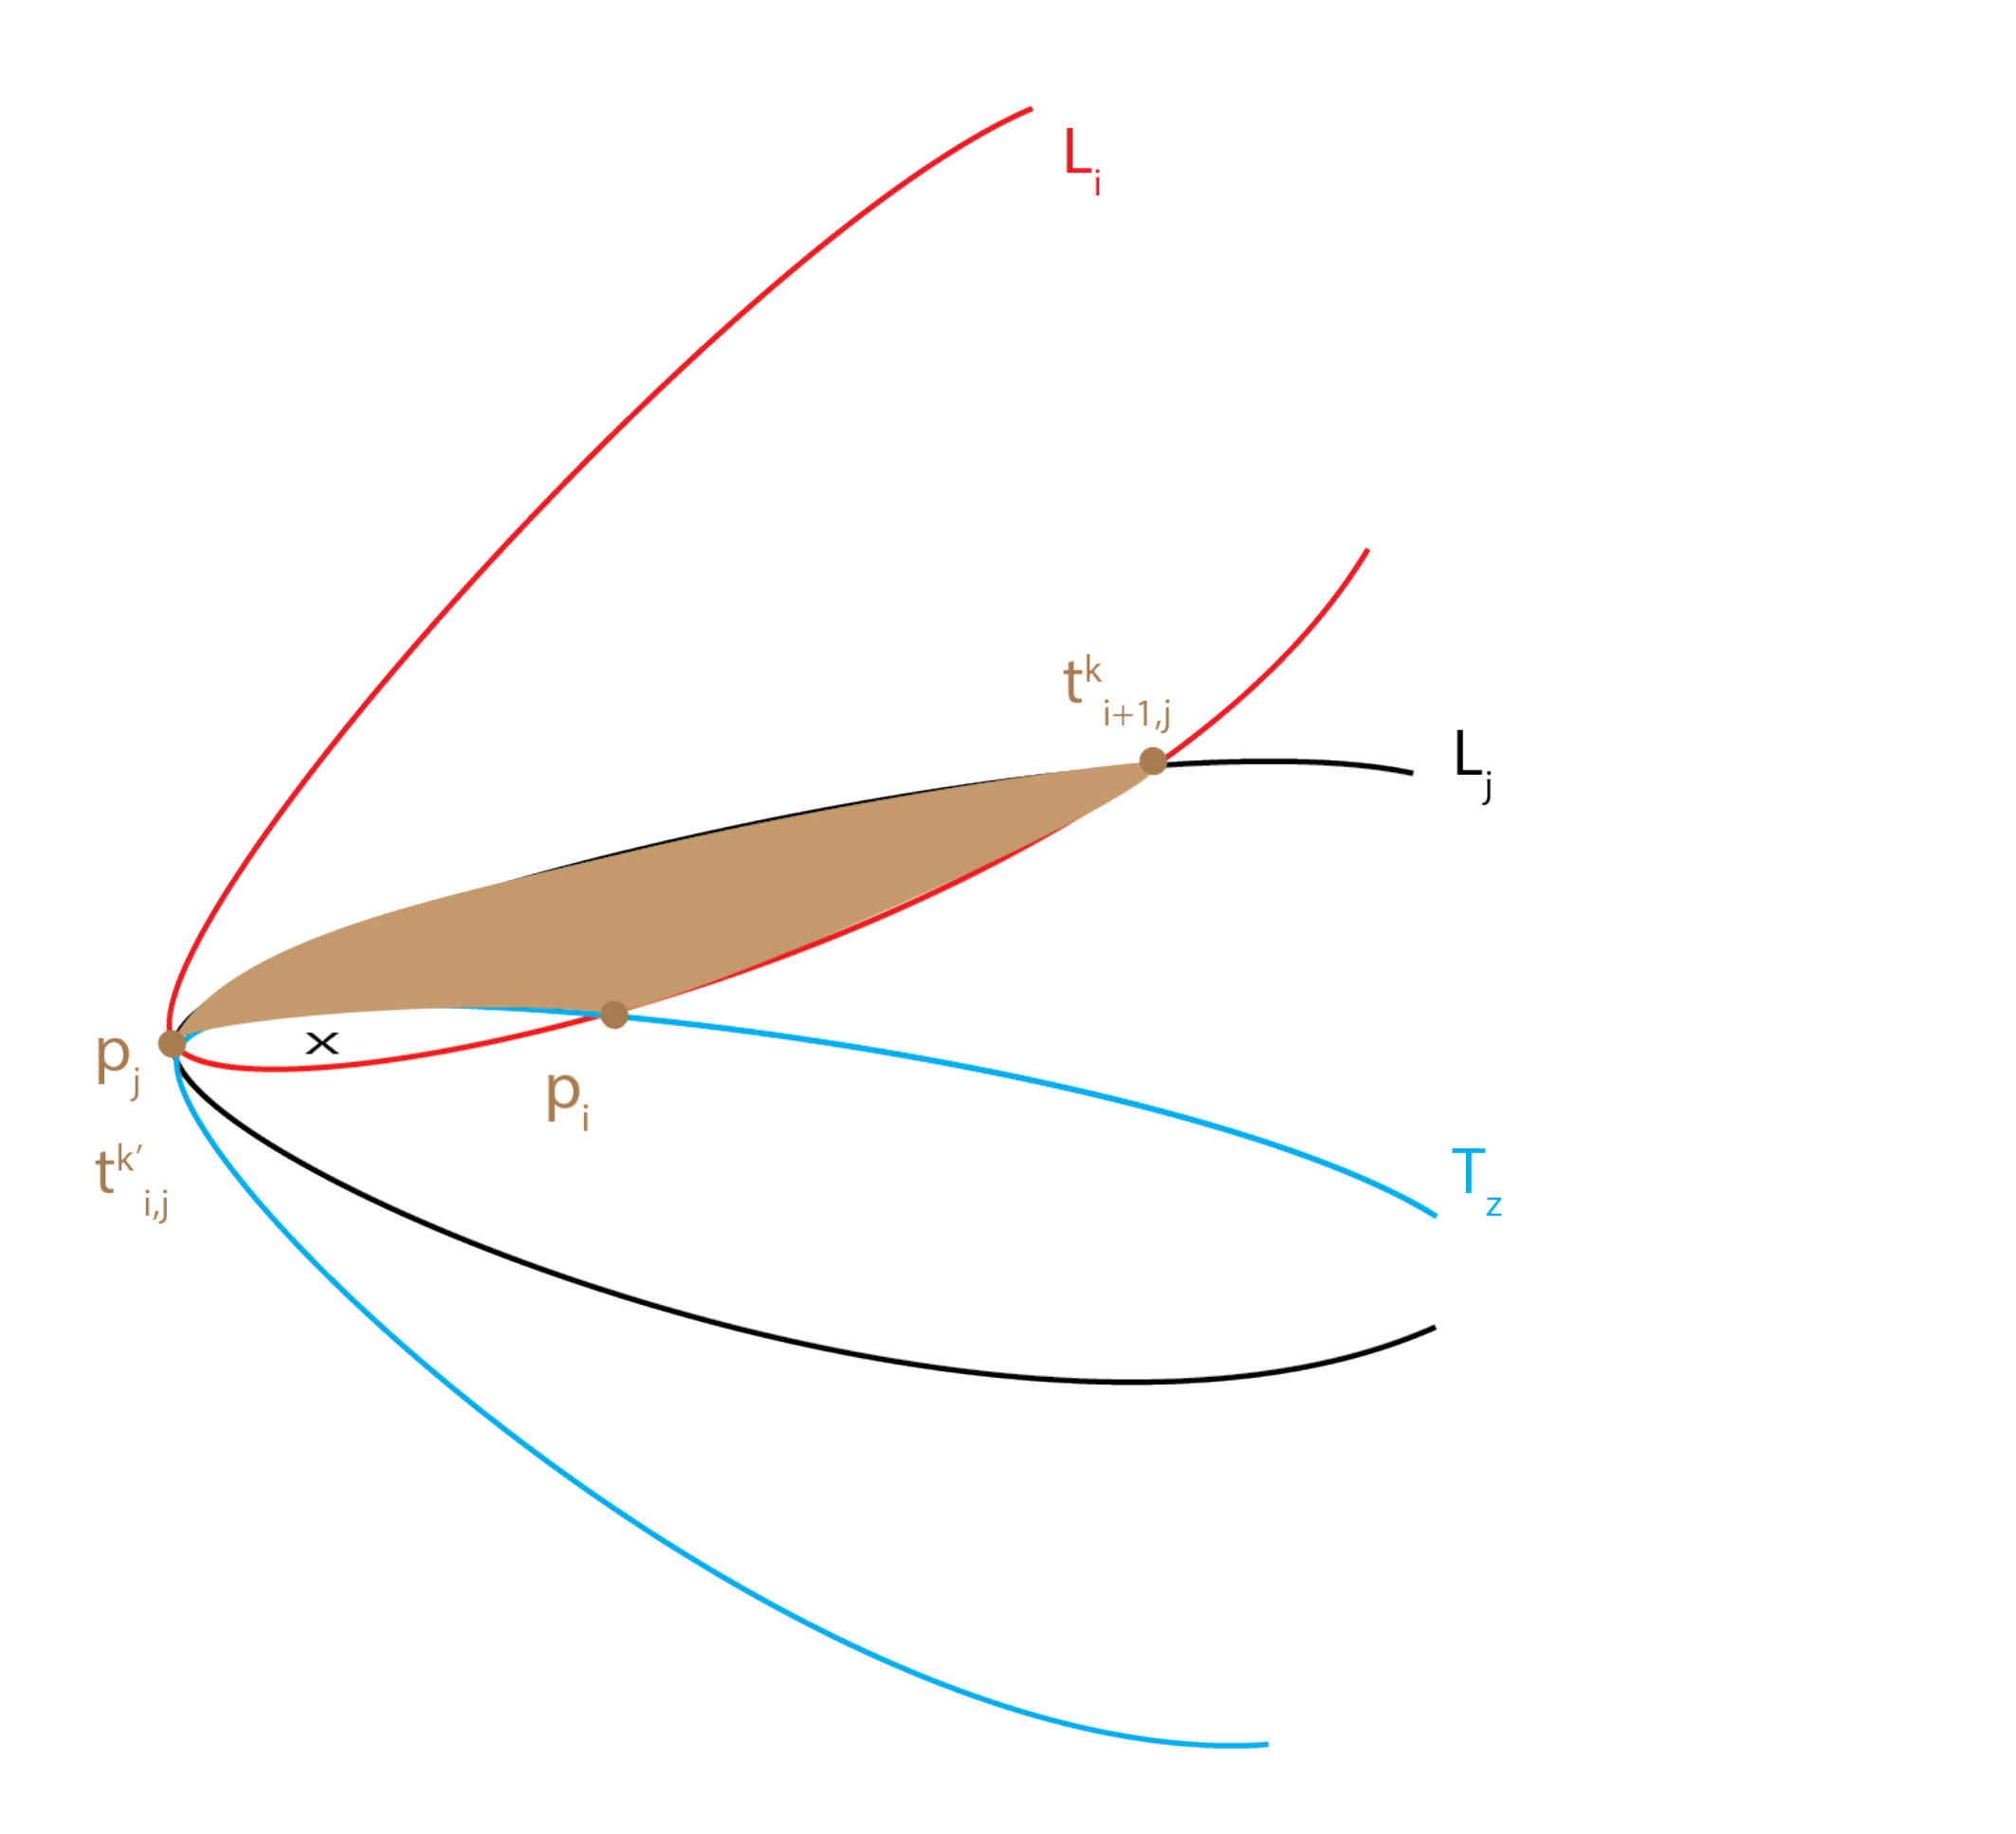
\includegraphics[width=0.40\textwidth]{figures/fig_5_1.png}
\caption{Leibniz 法则（原书 p.116）}\label{fig:leibniz}
\end{figure}

下面描述同伦论证，它将使我们求出 $M^1(p_i)$。见图 5.2 与 5.3。

\begin{figure}[!htbp]
\centering
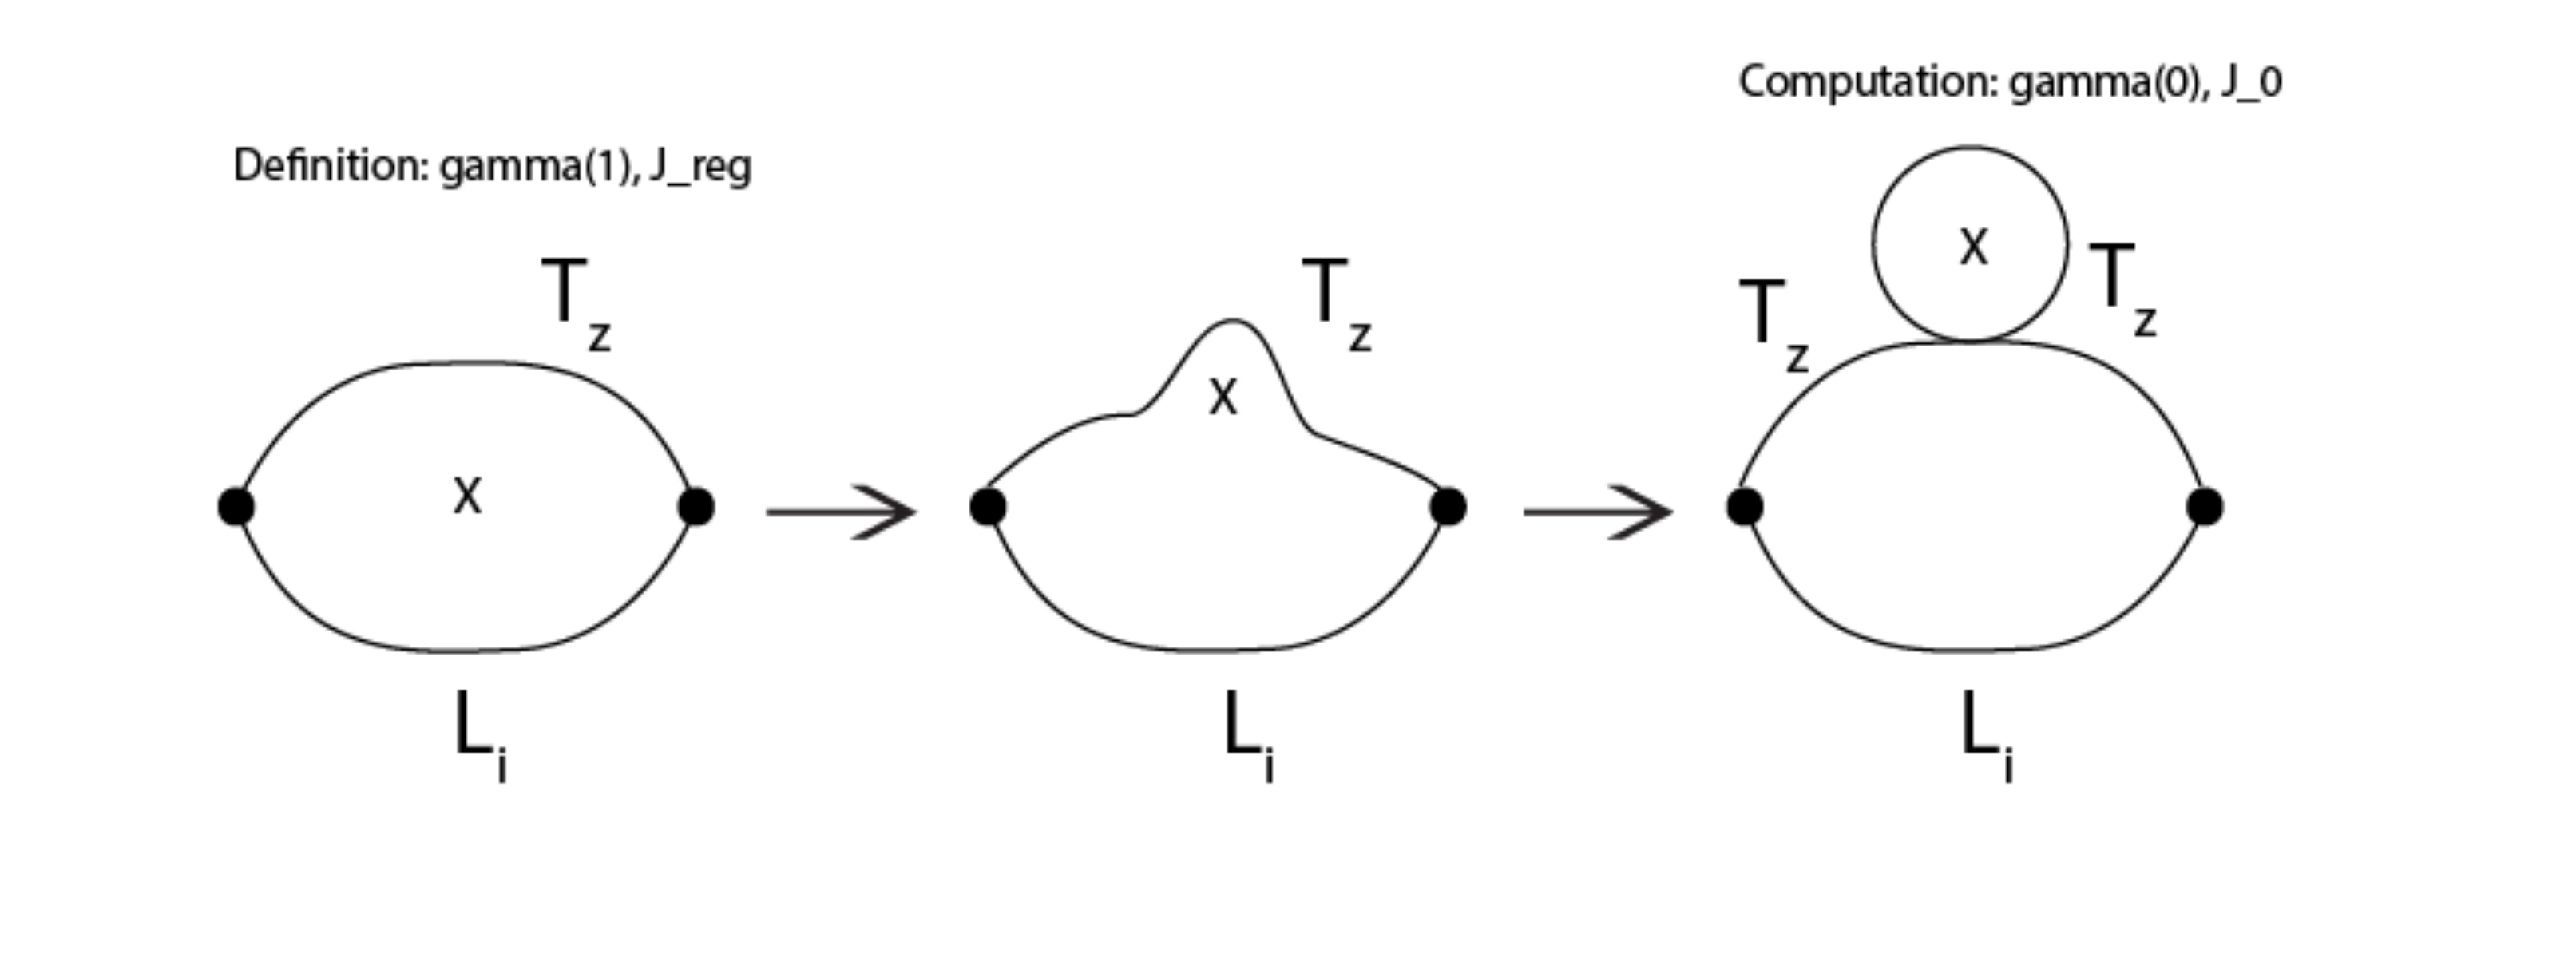
\includegraphics[width=0.84\textwidth]{figures/fig_5_2.png}
\caption{$\partial$（左）与我们所计算的圆盘计数（右）之间的同伦（原书 p.116）}\label{fig:homotopy}
\end{figure}

\transnote{图 5.2 左边标着「Definition: gamma(1), J\_reg」，右边标着「Computation: gamma(0), J\_0」。左图是定义侧：$T_z$ 与 $L_i$ 之间夹一个圆盘 $x$。右图是计算侧：同一圆盘在 $r=0$ 处多出一个球泡。两者之间的箭头表示同伦，而不是相等。}

\begin{remark}\label{rem:abstract-perturb}
用 $J_0$ 计算时，我们使用的是非正则 $J$。因此需要一套关于 $J$ 的不变性论证，它要涵盖非正则 $J$ 下的不变性。为此我们采用 polyfold 的抽象正则化方法：用 Banach 丛的一个截面扰动 $\bar\partial_{J_0}$；该截面未必由扰动 $J_0$ 诱导，故称「抽象」。
\end{remark}

[KL19] 中 Gromov--Witten 不变量的计算，需要证明开 Gromov--Witten 与闭 Gromov--Witten 具有同构的 Kuranishi 结构；

% ===== 原书 p.117 =====
\begin{figure}[!htbp]
\centering
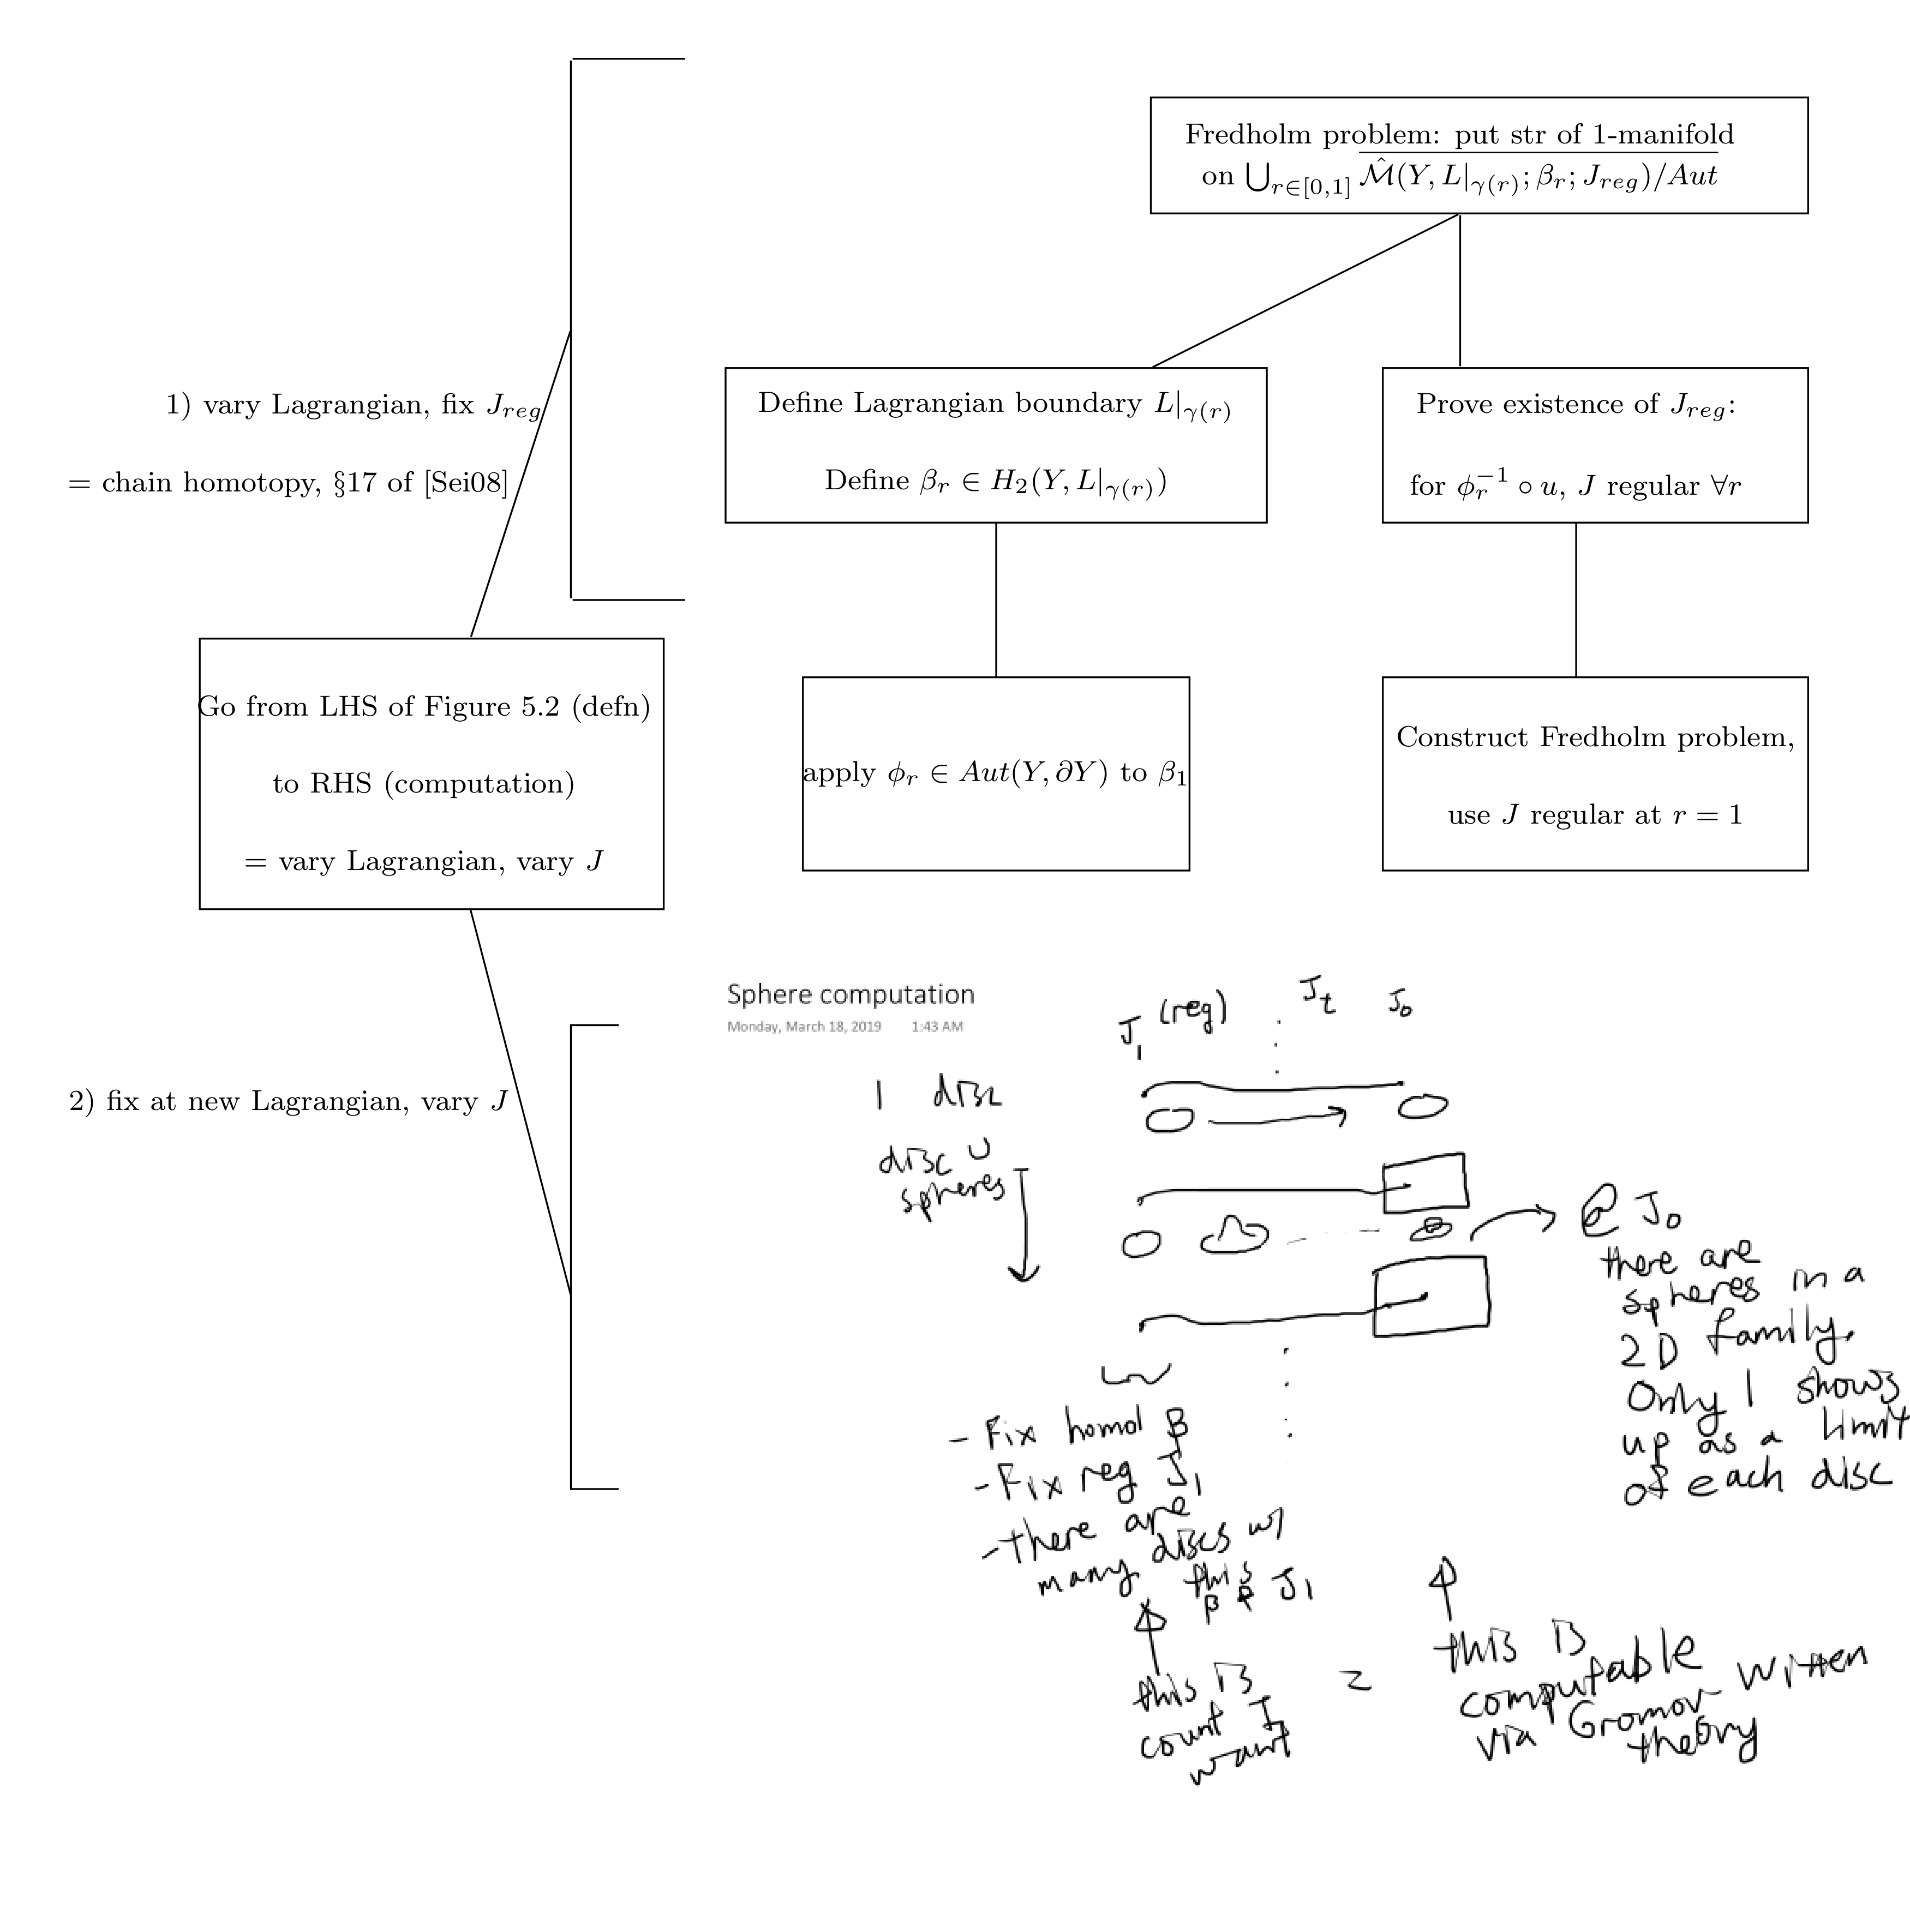
\includegraphics[width=0.46\textwidth]{figures/fig_5_3.png}
\caption{计算计划（原书 p.117）}\label{fig:plan}
\end{figure}

\transnote{图 5.3 是作者手写的流程图，页面上没有可排版的正文。图中左侧是两条路线：1）变拉格朗日、固定 $J_{reg}$；2）在新拉格朗日处固定，变 $J$。右侧上方是从 $J_{reg}$ 到 $J_0$ 的 Fredholm 问题构造，下方手写部分是球泡计算的草稿。中间的 $\widehat{\mathcal{M}}(Y,L|_{\gamma(r)};\beta_r;J_{reg})$ 表示带 $r$ 参数族的模空间。}

% ===== 原书 p.118 =====
这一点用到 [Cha11]，下文还会讨论。本节先讨论同伦论证；然后讨论圆盘与球泡的计算；最后用 polyfold 论证说明计算与定义的关系。

\begin{remark}[记号]\label{rem:notation-seidel}
本节使用 [Sei08, §17g] 中发展起来的理论，用于数穿过奇异纤维的伪全纯多边形截面。在该节中，$d$ 在这里称为 $M^1$。Seidel 的 $L_1,L_2$ 在本设定中为 $t_z$，且 $Q=\ell_i$；这由 $L_2$ 同痕于 $\phi(L_1)$ 得到。此处的其他映射应与 Seidel 的记号同名。
\end{remark}

\transnote{读本节必须同时翻开 [Sei08, §17g]。那里的 $d$ 是微分，此处改称 $M^1$；那里的 $L_1,L_2$ 是拉格朗日，此处是环面纤维 $t_z$；那里的 $Q$ 此处是 $\ell_i$。作者只保留了结构，不保留字母，稍不留神就会把两套记号混在一起。}

\begin{lemma}\label{lem:M1-homotopic}
$M^1:CF(T_z,L_i)\to CF(T_z,L_i)$ 同伦于 $M^2(c,-)$，其中 $c$ 是圆盘计数乘以合适的交点 $p$。
\end{lemma}

\begin{proof}
首先注意
\[
M^1:CF(t_z,\ell_i)\to CF(t_z,\phi(\ell_i))
\xrightarrow[\phi^{-1}]{C}F(\phi^{-1}(t_z),\ell_i)=CF(t_z,\ell_i)\cong\C,
\]
其中 $\phi$ 是单值性。这里用到：微分同胚 $\phi^{-1}$ 给出交点之间的双射；而 $t_z$ 在平行移动下不变，因为它只旋转角度。于是得到 $CF(t_z,\ell_i)$，而它只有一个交点。

开 Gromov--Witten 不变量理论可以数 $J_0$-全纯圆盘：边界在矩映射纤维上，有一个标记点，并且穿过 $Y$ 的奇异纤维一次（确实如此，因为按定义它们是 1-1 的，且在 $J_0$ 下实际得到 $v_0$ 的截面）。然而，$M^1$ 按定义是在 $T_z$ 与 $L_i$ 上边界、穿过奇异纤维的 bigon 计数。于是仿照 [Sei08, §17g]，我们形变 $M^1$。把边界在 $T_z$、标记点为 $p$ 的 $J_0$-全纯圆盘计数记为 $c\cdot p$。该形变构造同伦 $l$，使
\[
M^2(c,\cdot)-M^1(\cdot)=M^1\circ l-l\circ M^1=0,
\]
其中为零是因为在环面纤维上 $M^1=0$。见图 5.2。下面我们叙述他书中的细节，并按本文略有不同的设定补足所需信息。在本设定中，Seidel 作 Dehn 扭转所对的 vanishing cycle，其类比是三族退化为交于一点的 $S^1$ 的 $T^2$。不过，应用他的理论需要一条性质：单值性 $\phi$ 保持 $t_z=\{(\xi_1,\xi_2,\theta_1,\theta_2)\}_{\theta_1,\theta_2\in[0,2\pi)}$；这一点在这里仍成立。

我们先定义 $k$，它是 $\tilde d:=M^2(c,-)$ 与零映射之间的同伦；这里 $c$ 是闭的，从而是 Floer 同调的代表类。令 $\tilde l=M^2(k(\cdot),\cdot)+M^3(c,\cdot,\cdot)$。
\end{proof}

\begin{claim}\label{claim:boxed}
$(\tilde d,\tilde l)$ 满足 [Sei08, (17.15)] 中的框内方程；这些方程表示 $\tilde d$ 是纤维上两个 $CF$ 群之间的链映射，而 $\tilde l$ 是 $\tilde d\circ M^2$ 到零的同伦。
\end{claim}

此外，同痕 $L_1,L_2$，并取满足同一组方程的不同 $(d,l)$ 选择，所得映射彼此同伦。因此有唯一性陈述；取选择的极限不改变理论。

% ===== 原书 p.119 =====
\begin{proof}
方程 (17.15) 由 $(\tilde d,\tilde l)$ 的定义即得满足。下面看 $(d,l)$ 如何依赖 $L_1$，带 tilde 的情形同理。用 continuation maps $a$ 与 $b$，分别从 $CF(Q,L_1)$、$CF(L_0,L_1)$ 走到 tilde 版本。于是这些映射良定义，即输入相同。Seidel 还断言：continuation maps 与三角积相容，至多差一个链同伦。continuation maps 的模空间中的映射，其边界条件在 $Q$ 或 $L_1$ 上为常值，并在条状端的时间 1 侧实现 $L_1$ 到 $\tilde L_1$ 的同痕。三角积相容性所需链同伦 $h$ 的模空间如下：取边界为 $Q,L_0,L_1$ 的平凡纤维丛，粘上 $a$ 的模空间；对 $(Q,L_0,\tilde L_1)$ 同样做，粘上 $b$。链同伦 $h$ 定义为在这两者之间。由于 continuation maps 是拟同构，上同调上得到同构。同样，同痕 $L_2$ 仍得上同调同构。

先看插值于 Floer 复形之间的模空间。具体说，$\delta$ 是两端交点 $t_z\cap\ell_i$ 上两个 Floer 复形之间的映射；$\lambda$ 是积映射。新对象 $\delta,\lambda$ 满足与 (17.15) 类似的方程，但分别多出 $d+\tilde d$ 与 $l+\tilde l$ 项。这些方程说的是：链复形 $C'\oplus C\oplus C''$ 与 tilde 版本同构。注意 $(\delta,\lambda)$ 是更一般地变 $(\tilde d,\tilde l)$ 的构造；而 $(\alpha,\beta)$ 是特别地通过变 $L_1$ 来变 $d$ 的构造，后者比前者引入更多项。

再看为何满足 (17.15) 的不同 $(d,l)$ 选择给出同伦的结果（这比「同痕 $L_1,L_2$ 得到不同选择」更一般）。取这样的 $(d,l)$。我们构造 $d$ 与 $\tilde d\circ a$ 之间的同伦，记为 $\alpha$；同样，记 $\beta$ 为 $l$ 与 $\tilde l$ 之间的链同伦。continuation maps 是拟同构，而 $\alpha,\beta$ 给出 $D$ 与 $\tilde D$ 之间的映射，它也是拟同构。
\end{proof}

\begin{claim}\label{claim:compute-M1}
我们可用 $M^2(c,-)$ 计算 $M^1$，并得到拟同构的 Fukaya 范畴。
\end{claim}

\begin{proof}
这是唯一性陈述的极限情形。这里 $\xi$ 与 $\psi$ 分别对应变微分与变乘积；$\xi$ 在 Seidel 所称的 $d$ 与 $M^2(c,-)$ 之间插值。我们取 $L_1$ 上同痕的极限。理由是：上一节正是这样变 $L_1$ 的，因此也正是这样变 $d$ 的。于是 $\tilde d$ 是上一节的极限情形，因为它是同痕 $\tilde L_1$ 的极限情形：这里 $\tilde d=M^2(c,-)$。
\end{proof}

% ===== 原书 p.120 =====
现在构造三角积的不同选择之间的同伦：考察一个由五部分组成的参数族。第一部分是原 $(d,l)$ 对中的 $l$。第二族关联于 $\xi(M^2)$：把 $\xi$ 纤维丛粘到一个平凡的 3 点圆盘。回忆 $\xi$ 是插值于两个「类微分」选项 $d$ 与 $M^2(c,-)$ 之间的 1 参数族。于是把这个族粘到 3 点圆盘上，又得到一个族。这样做实际上是把 $\xi$ 族变成作用于乘积层面的族。「大粘合长度」意味着它就是 $\xi(M^2)$。注意在 $r=0$ 处得到 $r=1$ 的 $l$ 族。在第二 $\xi$ 族的另一端，当 $r=1$ 时得到 $M^2(c,M^2(,))$。取足够大的闭区间 $[0;1]\subset\R^4$。
% [Tutor Note: 原文作 [0; 1] ⊂ R^4，与上下文不合；疑为 [0,1] ⊂ R 或 [0,1]^4 之误。译文保留原样，登记于报告。]

\transnote{原文此处作「$[0;1]\subset\R^4$」，分号与 $\R^4$ 都显得突兀。按上下文，作者只是要一个足够大的参数区间，故疑为 $[0,1]\subset\R$ 或 $[0,1]^4$ 的笔误。译文保留原样，未作改动。}

\begin{remark}\label{rem:gluing}
同伦的一侧有映射复合，即 $M^2(c,-)$。Fukaya 范畴中两个结构映射复合时，几何上对应把产生各自模空间的 Fredholm 问题粘起来。因此本设定下需要讨论粘合。这也是本设定与 Seidel 不同之处：书中他形变纤维丛；而此处丛不变，变的是拉格朗日边界条件。于是需要粘合论证，以推出模空间
\[
\bigcup_{r\in[0,1]}\mathcal{M}(J_{reg},L_r)
\]
是一维光滑流形。以下理论依照 [Weh14, Lecture 9]；另见 Wehrheim 2013 年秋季 topics 课程第 14 讲及 McDuff--Salamon：先用 $J_z$ 做，§10.9 处理只有 $J$ 的情形。
\end{remark}

\begin{claim}\label{claim:1dim}
$\displaystyle\bigcup_{r\in[0,1]}\mathcal{M}(J_{reg},L_r)$ 是 1 维流形。
\end{claim}

\begin{proof}[证明梗概]
为证光滑结构存在，构造一个 Fredholm 问题。设 $\gamma_r$ 为图 5.2 所示纤维丛底空间中的变动路径。设 $\{\phi_r\}_{r\in(0,1]}$ 是微分同胚的同痕
\[
\phi_r:(Y,L_i\cup T_z|_{\gamma_1})\xrightarrow{\cong}(Y,L_i\cup T_z|_{\gamma_r}),
\]
它在相应的相对第二同调群上诱导同构 $\phi_{r*}$。注意当 $r=1$ 时，用上面的方法已有曲线模空间的正则 $J$，且几何条件允许排除泡泡，于是得到紧的一维空间。这个 $J$ 又让我们定义一个 Banach 丛，作为 Fredholm 问题的底：
\[
\tilde{\mathcal{B}}^{k,p}:=\{(\phi_r^{-1}\circ u,r)\mid u:\R\times[0,1]\to(Y,L_i\cup T_z|_{\gamma_r})\in W^{k,p}\}.
\]
\end{proof}

% ===== 原书 p.121 =====
换一种说法，可把 $\tilde{\mathcal{B}}$ 中一条路径的切空间刻画为：路径在边界处的导数等于一个向量，该向量是拉格朗日边界切空间中的向量与同痕 $\phi_r$ 的流向量之和。由此，满足 $\bar\partial_J(\phi_r^{-1}\circ u)=0$ 的映射 $u$ 之集合得到 1 维流形结构，其中 $J$ 是上面定义的正则 $J$。

下一步在 $r=0$ 端作 Gromov 紧化。注意 $\phi_r$ 在 $r=0$ 处没有极限：它变得高度退化，不再是微分同胚。所以我们改把模空间中的元素看作 $u$，而不看作 $\phi_r^{-1}\circ u$。然后修改粘合论证，把 $r=0$ 处的两个同调类粘起来，使粘好的曲线成为 $r>0$ 曲线的极限。反过来，由 Gromov 紧性论证可以重参数化，推出 $r>0$ 映射的极限正是图 5.2 所示的三角形粘到圆盘上。更具体地说，见下文。

\medskip\noindent\textbf{粘合区域}\par
预粘合的做法是：在要粘合处的一个邻域内平凡化法丛，然后在两个映射之间线性插值。见 [Weh14, lec 3, 1 hr]。注意即使不做平凡化，法丛上也有缩放函数。取 $r$ 为底空间中两个圆盘的粘合参数；它将是颈部周围四个点的交比，而颈部正被掐成一点。注意粘合参数为 $e^{-\ell}$，当粘合长度 $\ell$ 趋于无穷时它趋于零，这就是两个圆盘的构型。

我们如下预粘合区域。先去掉 puncture 的一个邻域。在条状端的 $(s,t)$ 坐标中，把 $(s-\ell,t)$ 粘到 $(s,t)$。也就是说，在一个条带上沿 $\R$ 方向放一段长度 $\ell$，重叠到另一条带上。两部分分别给出 $r=0$ 的情形；两部分粘在一起则给出 $r=\epsilon>0$ 的情形。给出条状端嵌入的映射如下：1）用乘以 $\pi$ 把 $(-\infty,0]\times[0,1]$ 映入 $(-\infty,0]\times[0,\pi]$；2）再用 $e^{-z}$ 映入圆环的下半部分；3）最后用 $\frac{z+i}{z-i}$ 映入在 $1$ 处有一个 puncture 的圆盘的右半部分。预粘合映射之所以接近 $J$-全纯的粘合映射，是因为由连续性，粘合映射的 $\bar\partial_J$ 仍然很小；若它在粘合部分为常值，则实际上全纯。由于我们缓慢插值，它确实接近常值。注意存在 Gromov 拓扑，它在此空间上给出距离度量；而可度量化空间是 Hausdorff 的。

接着对预粘合圆盘作 Newton 迭代，以得到 $J$-全纯曲线。粘合过程如下：在预粘合映射处，对拉回切丛取指数映射，在纤维中可以相加向量。切向量 $\xi$ 由 Newton 迭代得到（这是压缩映射原理的论证），它在 Banach 空间上适用。

% ===== 原书 p.122 =====
我们的几何设定保证：对每个 $0<r\le1$，$J$-全纯圆盘的模空间不会极限到圆盘泡、条断裂或球泡。在 $r=0$ 处确实会形成一个圆盘泡，由 Gromov 紧性可知这必然发生。也就是说，我们作紧化，把边界上的纤维积作为 Fredholm 截面的零点集。注意我们也能找到在 $r=0$ 构型处同样正则的 $J$。我们在每个圆盘分量上用通常的 $\bar\partial$ 算子，并在两赋值映射应当相遇处取其差。这同样有 Fredholm 设定，参看 [Weh14, Lecture 3, 22 mins]。

此后，我们考虑把映射粘到 $v_0:Y\to\C$ 的底空间上，而不只是像上面那样粘区域；最后用矩映射坐标 $(\xi_1,\xi_2,\eta,\theta_1,\theta_2,\theta_3)$ 把映射 $u$ 粘到全空间。

于是得到 $r=0$ 与 $r=1$ 两种选择之间的紧一维配边结构。

这就完成了证明：$M^1$ 与 $M^2(c,-)$ 之间的同伦良定义，它是一维模空间的边界。

\medskip\noindent\textbf{圆盘的计算}\par
本节取 $J=J_0$，只考虑圆盘的模空间；对这些模空间 $J_0$ 是正则的。换言之，我们只考虑来自圆盘的同调类 $\beta$。注意：对所有构型都正则的 $J$ 之集合非空且稠密，而映射在零点的一个邻域之外是 $J_0$ 截面；由正则 $J$ 的稠密性，可以断言 $J_0$ 是这类 $J$ 的极限。也就是说，有一串 $J$ 收敛到 $J_0$，这些 $J$ 只在零纤维附近扰动 $J_0$。见 5.3 中的球图。

\transnote{「$J_0$ 是正则 $J$ 的极限」这句话是本节所有计算的合法性来源。作者并不是直接在 $J_0$ 上数圆盘，而是把 $J_0$ 看作一列正则 $J$ 的极限，再用不变性把计数搬到 $J_0$。若忽略这一层，会把「$J_0$ 下不正则」与「不能计数」混为一谈。}

\begin{remark}\label{rem:M0}
若把绕 $v_0:Y\to\C$ 的底空间一圈平行移动所得的 $t_z$ 作为拉格朗日纳入所考虑的子范畴，则这个拉格朗日界定非常值的全纯圆盘。一个未来的方向是把它纳入，并为包含该拉格朗日的范畴定义 $M^0$。注意 $M^0$ 在 $\Z/2$ 中的指标为 2。本文不把它纳入所考虑的子范畴。我们仍然要数圆盘与 $J_0$-球，但它们只出现在 $M^2(c,-)$ 的 $c$ 中，而 $M^2(c,-)$ 看作 Floer 群上的映射。
\end{remark}

以下内容依据 [Aur07] 与 [CO06]。

\begin{definition}[拉格朗日的 Maslov 类]\label{def:maslov}
$HF(L_0,L_1)$ 有 $\Z/N$ 分次，至多差平移。可以取相对分次（至多差平移），也可以取绝对分次（无平移）。例如 $N=2$。设 $2c_1(M)=0$，于是反典范丛的平方可由某个截面 $s$ 平凡化。
\end{definition}

% ===== 原书 p.123 =====
对每个拉格朗日的基取 $\det^2$，得到从 $LGr$ 到 $K^{-2}$ 的单位丛的映射。用上述平凡化截面 $s$，可把这个单位丛等同于 $S^1$。结果得到映射 $LGr\to S^1$。「Maslov 类」就是 $[S^1]$ 的拉回，于是得到 $LGr$ 中的一个同调类。

\begin{lemma}[{[Aur07, §3.1]}]\label{lem:maslov}
设 $(X,\omega,J)$ 是光滑、紧的凯勒流形。设 $\Omega\in\mathcal{M}^0(X,(T^{*(1,0)}X)^n)$ 是全局亚纯 $n$-形式，其极点沿反典范除子 $D$（例如用对数坐标）。换言之，$\Omega^{-1}$ 是 $X\setminus D$ 上反典范丛的非零全纯截面。

设 $L$ 是 $X\setminus D$ 中的拉格朗日子流形，且是特殊的，即 $\Omega|_L$ 在局部全纯坐标函数中辐角为常值。设 $\beta\in\pi_2(X,L)$ 非零。

则：对这个特殊拉格朗日 $L$，$M(\beta)$ 是代数相交数 $\beta\cdot[D]$ 的两倍。
\end{lemma}

\begin{proof}
$L$ 的切空间是实的，因为拉格朗日的定义是 $(TL)^\perp=JTL$（关于 $\omega(-,J-)$）。取一组实基，得到 $K_X^{-1}|_L$ 的一个非零截面；可把它缩放到单位长度。由于已归一化，这个截面与基的选择无关。特别地，它的平方平凡化反典范丛的平方，即 $2c_1(X\setminus D)=0$。也就是说，回忆 $M(\beta)$ 度量的是：把 $L$ 上这个归一化截面的平方延拓到代表 $\beta$ 的圆盘上的障碍。由 [Sei00]，我们总可以得到分次 $M$，因为对特殊拉格朗日有到 $\R$ 的提升，如下。最终 $TL$ 上有两个非零的单位实截面，故二者必相同；其中之一是（对应除子 $D$ 的）截面的平方。于是 $\beta$ 的 Maslov 类，经由这个平方截面，等于 $D$ 与 $\beta$ 的相交数的两倍。
\end{proof}

\begin{theorem}[{[CO06], [Aur07]}]\label{thm:dimension}
考虑边界在 $L$ 中、属于类 $\beta$ 的 $J$-全纯圆盘的模空间。其虚拟维数为 $n-3+M(\beta)$。断言是：这些模空间中各有一个圆盘。
\end{theorem}

\begin{proof}
维数断言的依据是：由 Fredholm 理论，维数应为 $M(\beta)$；但随后要加上 $n$ 个标记点，并减去重参数化的作用（3 点决定圆盘的一个自同构）。
\end{proof}

从维数上我们预期：由于看的是截面，它们穿过中心纤维，而中心纤维也是除子 $D$。它们与 $D$ 横截相交一次，故 Maslov 指标为 2。然后假设有一个边界标记点。于是期望维数为：Maslov 指标贡献 2，加上标记点贡献 1，再减去商掉重参数化的 3，结果期望维数为零。（边界在 $T_z$ 上、并固定边界上一点的圆盘是零维族；否则可用 $T^3$ 作用旋转圆盘，得到一族圆盘。固定边界点把维数降到零，从而可以计数。）

% ===== 原书 p.124 =====
$T_z$ 可看作对应点层（skyscraper sheaf）。回忆此前 $\ell_i$ 的含义：沿角度方向旋转，在底空间每个矩映射方向绕一圈。只在角度方向旋转、不在底空间旋转，就得到 $T_z$。具体说，固定矩映射坐标、让角度变化。这给出矩映射坐标 $A=(a_1,a_2,a_3)$ 的原像；令 $z=e^{2\pi iA}$ 为指数化坐标。选用字母 $A$ 的理由是：这类圆盘的计数公式在 [CLL12] 的一篇文中讨论过，而其记号与这里一致。

回忆 $Y$ 作为环簇带有复坐标，因此带有自然的 $J_0$。额外的复杂之处在于它有全纯球。这将在下文考虑。我们将描述 $J_0$ 下出现的圆盘，证明该计数与 theta 函数相符；然后讨论变 $J_0$ 的几何正则化论证，用指标与维数理由排除邻近 $J$ 下球的存在。

带 1 个标记点的圆盘模空间的复维数为：标记点贡献 1，减去自同构群的 3，再加上圆盘类 $\beta$ 的 Maslov 指标。我们要维数为零，故要求 $1-3+2\beta\cap D=0$；这里回忆 Maslov 指标 $M(\beta)=2\beta\cap D$，而 $D$ 是 $v_0^{-1}(0)$ 中环簇除子之并。于是 $\beta\cap D=1$ 意味着我们只需考虑与中心纤维相交一次的 Maslov 2 圆盘。没有非常值的 Maslov 0 圆盘，因为纤维中的拉格朗日不界定圆盘。

我们可以在卡 $\C^*\times\C^*\times\C$ 中看这个圆盘（拉回到万有覆盖；由环簇几何知 $\pi=1$）。于是，边界在 $S^1(r_1)\times S^1(r_2)\times S^1(r_3)$ 中的圆盘不能出现在前两个分量上（由极值原理），从而得到最后一个 $v_0$ 坐标中的圆盘。它不能多重覆盖，因为 Maslov 指标 2 既是最小值也是最大值。所以我们数的圆盘对应于：在矩多面体中取一点 $A$，画一条线到某个面，这意味着 $|v_0|$ 降到 0。

\begin{theorem}\label{thm:disc-count}
圆盘计数等于定义 theta 函数，至多差一个坐标变换。
\end{theorem}

\begin{proof}
回忆计数中以 $e^{-\int\omega}$ 加权；现在显式求出面方程。
\end{proof}

在 3 维中，我们得到面方程
\[
\left\langle\nu(F_{m_1,m_2}),\begin{pmatrix}\xi_1\\ \xi_2\\ \eta\end{pmatrix}\right\rangle
+\alpha(F_{m_1,m_2})
=\langle-m_1,-m_2,1\rangle\cdot\langle\xi_1,\xi_2,\eta\rangle
+m_1^2+m_2^2+m_1m_2=0.
\]

% ===== 原书 p.125 =====
而两个级数为（其中 $x_i$ 是 $V$ 复侧的坐标，$z_i$ 是 $e^{2\pi i a_i}$；多面体中所量的点为 $(a_1,a_2,a_3)$，面积为 $2\pi(\langle a,\nu(F_{m_1,m_2})\rangle+\alpha(F_{m_1,m_2}))$，或带 $T$ Novikov 参数）：
\[
\theta\text{-function}=\sum_{n\in\Z^2}x_1^{n_1}x_2^{n_2}e^{\frac12 n^T\begin{pmatrix}2&1\\1&2\end{pmatrix}n},
\]
\[
\text{按面积的圆盘计数}=z_3\sum_{n\in\Z^2}z_1^{n_1}z_2^{n_2}e^{\frac12 n^T\begin{pmatrix}2&1\\1&2\end{pmatrix}n}.
\]

把原点移到多面体中瓦片的中心，即可消去 $m_1,m_2$ 的附加项。$(m_1,m_2)$ 瓦片的法向为 $\langle-m_1,-m_2,1\rangle$。在 $(m_1,m_2)$ 处，瓦片沿 $(1,0)$ 方向移动意味着加上 $\langle2,1,z\rangle$；它必须垂直于 $\langle-m_1,-m_2,1\rangle$，故 $z=2m_1+m_2$。同样，从 $(m_1,m_2)$ 瓦片沿 $(0,1)$ 方向移动，加上 $\langle1,2,m_1+2m_2\rangle$。要求每个面的方程，除了法向，还需要六边形上的一点。取左下角；在 $(0,0)$ 瓦片中它从 $(-1,-1,0)$ 开始。我们刚求出它沿每个方向如何增加。

于是，从 $(0,0)\to(1,0)\to\cdots\to(m_1,0)$ 瓦片，依次加上 $\langle2,1,0\rangle$、$\langle2,1,2\rangle$，直到 $\langle2,1,2(m_1-1)\rangle$，故总计为 $\langle2m_1,m_1,m_1(m_1-1)\rangle$。再从 $(m_1,0)$ 瓦片到 $(m_1,1)$ 瓦片，加上如上所得的 $\langle1,2,m_1\rangle$，依次类推，最后到 $\langle1,2,m_1+m_2(m_2-1)\rangle$。故总共增加 $\langle m_2,2m_2,m_1m_2+m_2(m_2-1)\rangle$。因此我们的特征点为
\[
\langle2m_1+m_2-1,\ m_1+2m_2-1,\ m_1(m_1-1)+m_2(m_2-1)+m_1m_2\rangle,
\]
而我们知道它满足
\[
\langle-m_1,-m_2,1\rangle\cdot\langle\xi_1,\xi_2,\eta\rangle+\alpha(F_{m_1,m_2})=0.
\]
解之得 $\alpha(F_{m_1,m_2})=m_1^2+m_1m_2+m_2^2$，或
\[
\frac12 m^T\begin{pmatrix}2&1\\1&2\end{pmatrix}m
=\frac12 m^T(2m_1+m_2,\ m_1+2m_2)
=m_1^2+m_1m_2+m_2^2,
\]
这与 theta 函数相同。

\transnote{矩阵 $\begin{psmallmatrix}2&1\\1&2\end{psmallmatrix}$ 不是凭空出现的：它的元素是两个瓦片移动向量的内积，也可以理解为该二次型的 Gram 矩阵。第 125 页的推导正是要说明：面方程中的 $\alpha$ 恰好等于这个二次型，因此按面积加权的圆盘计数逐项等于 theta 级数。}

\begin{remark}\label{rem:finish-plan}
我们完成图 5.3 中计算计划的剩余部分。在 $J_0$ 下、同调类中没有 $\alpha$ 球时，由不变性知模空间中有 1 个圆盘。$J_0$ 下各个圆盘自身都是正则的。然后看 $J_t$-全纯圆盘 $u_t$ 当 $t\to0$ 时的极限；也就是说，它们解 $J_t$ 的 Cauchy--Riemann 方程。
\end{remark}

% ===== 原书 p.126 =====
在可能取子列之后，$\lim_{t\to0}u_t=:u_0$ 在 Gromov 拓扑下存在。由 Gromov 紧性并排除圆盘泡与条断裂，可知 $u_0$ 或是一个圆盘，或是圆盘并上一些球。这在 [CLL12, Proposition 4.30] 中讨论过。特别地，本应可能像上面变选择找链同伦那样，得到二者之间的代数关系。但我们改用 polyfold 理论，在已有计数之后证明良定义性；它擅长处理非正则 $J$，办法是对 $\bar\partial_J$ 算子作抽象扰动。

\begin{remark}\label{rem:more-discs}
$J$ 下的圆盘比 $J_0$ 下多，因为有些圆盘在 $J$ 下必须收敛到 $J_0$ 下的圆盘并泡。[MS12] 讨论了变 $J$ 时映射的变化。而在本设定中，变拉格朗日时同调类也变。用不变性：要得到 $J$ 下的模空间，只需对 $J$ 施加作用；然后利用 Fukaya 范畴与 $J$ 的选择无关这一性质。
\end{remark}

\medskip\noindent\textbf{$J_0$ 下球泡的计算：Gromov--Witten 不变量}\par
\begin{claim}\label{claim:nonregular-spheres}
存在对 $J_0$ 不正则的球。
\end{claim}

见 [Aur07, §4]。远离 0 上除子的 $T^3$-轨道，关于 $\wedge_i d\log x_i$ 形式是特殊拉格朗日。注意：若 $J$ 可积，则 $\bar\partial_J$ 复线性，故导数 $Du$ 相同。于是对没有 $(0,2)$ 形式的东西（例如本情形中源空间为黎曼面时确实如此），其余核恰是一个次数为 1 的 Dolbeault 上同调群。若它不为零，则不满射。因此零上的那些问题球泡不正则。指标算子给出 $n-3+c_1$，即 $2-3+0=-1$；维数 $-1$ 本不该出现，若出现就意味着这些球不出现——但我们知道它们确实出现，所以它不可能正则。它们出现在更高维的族中，故不是期望维数。变 $J_t$ 时，只有部分构型作为模空间的极限出现。

\begin{corollary}\label{cor:equivariance}
由等变性，本设定中出现一个常数因子，它不影响所得 Fukaya 范畴的拟同构类。
\end{corollary}

\begin{proof}[证明]
等变性在 [KL19] 中讨论。此外，任何产生这些模空间的设定都在群作用下不变。注意 [KL19] 定义的环簇凯勒形式与这里不同，但复结构（即 $J_0$）相同。我们将计算无限型环簇边界中球的面积。因此不同的辛形式只意味着 $\C\PP^1$ 可被不同地缩放。变辛参数会把 Gromov--Witten 理论中出现的凯勒参数纳入进来，[KL19] 称之为 $q$。由于这里固定辛形式，我们也就固定了凯勒参数 $q_i$。
\end{proof}

\medskip\noindent\textbf{球计数证明的思路}\par
下图给出理解 [KL19] 中球计数所需的背景。注意他们所用 $J=J_0$，与这里相同。

% ===== 原书 p.127 =====
\begin{center}
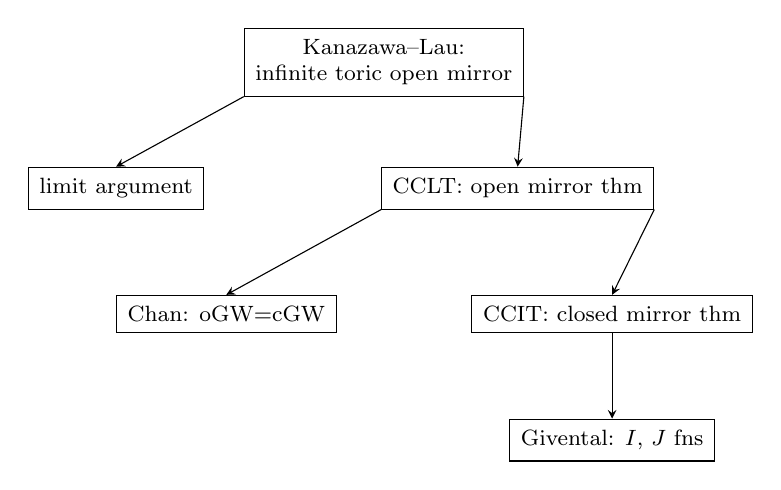
\begin{tikzpicture}[
  box/.style={draw, fill=white, inner sep=4pt, font=\footnotesize, align=center},
  arr/.style={->, >=stealth, thin}]
\node[box] (kl) at (0,0) {Kanazawa--Lau:\\infinite toric open mirror};
\node[box] (limit) at (-3.4,-1.6) {limit argument};
\node[box] (cclt) at (1.7,-1.6) {CCLT: open mirror thm};
\node[box] (chan) at (-2.0,-3.2) {Chan: oGW=cGW};
\node[box] (ccit) at (2.9,-3.2) {CCIT: closed mirror thm};
\node[box] (giv) at (2.9,-4.8) {Givental: $I$, $J$ fns};
\draw[arr] (kl.south west) -- (limit.north);
\draw[arr] (kl.south east) -- (cclt.north);
\draw[arr] (cclt.south west) -- (chan.north);
\draw[arr] (cclt.south east) -- (ccit.north);
\draw[arr] (ccit.south) -- (giv.north);
\end{tikzpicture}
\end{center}

\begin{lemma}[Givental]\label{lem:givental}
Picard--Fuchs 可计算 GWI，并且镜像于 Hodge 结构中周期的组合概念。Givental 引入了 $I$ 函数与 $J$ 函数。
\end{lemma}

\begin{remark}[闭镜像定理：{[CCIT15]}]\label{rem:closed-mirror}
我们提供一组资源，以说明理解 Gromov--Witten 不变量的时间线与背景。一侧的 $J$ 函数（Gromov--Witten 不变量）对应另一侧的 $I$ 函数（组合的）。这建立在 Givental 的工作上：镜像映射是 $1/z$ 的系数。见 [CK99, §6.3]。凯勒模与复模同构；镜像映射在凯勒大极限点的邻域与复侧的极大单值性之间。Picard--Fuchs 用于极大单值性附近的复模，[CK99] 记作 $y_k$；而 $q_k$ 用于凯勒模。GKZ 系统见 [CK99, §5.5]，Picard--Fuchs 见 §5.1.2。变复模给出 Hodge 结构的变分。§2.6.2 引入 Givental 的 $I,J$ 函数。§11.2.5 是环簇完全交的 Givental 镜像定理。第 10 章：模空间的 stack 定义。方程 (10.4) 给出微分/相交论与 GW 的关系。stack 入门的参考是 [Fan01]。[CK99, Proposition 10.3.4] 给出 $J$ 函数与 GW 势的关系。镜像定理的例子：11.2.1.3。Theorem 10.3.5：QM 微分算子当且仅当 Picard--Fuchs 算子。第 7 章给出 GW 的定义。$1/z$ 系数的陈述：[CK99, page 151]，[KL19] 中的 $z$ 即 [CK99] 中的 $y_0$。注意：据 [CK99]，Givental 镜像定理的等变性在原论文 [Giv98] 中并不完整；这正是 [CCIT15] 所讨论的。随后 [CCLT16] 加入 [Cha11] 的结果：
\[
M_X^{open}(\beta+\alpha)=M_X^{closed}(\beta+\alpha).
\]
等变性在 [CCIT15] 中讨论，因为那里是环簇设定。
\end{remark}

% ===== 原书 p.128 =====
\begin{definition}[Kuranishi 结构]\label{def:kuranishi}
$p$ 的 Kuranishi 邻域具有以下性质：
\begin{itemize}[leftmargin=2.2em,itemsep=0.25em]
\item $V_p$ 是光滑有限维\emph{流形}，可带角；
\item $V_p\times E_p\to V_p$ 称为\emph{障碍丛}（$E_p$ 是有限维实\emph{向量空间}）；
\item $\Gamma_p$ 是有限\emph{群}，光滑且有效地作用在 $V_p$ 上（无非平凡元素平凡作用），并在 $E_p$ 上线性地表示该群；
\item \emph{Kuranishi 映射} $s_p$ 是 $V_p\times E_p$ 的光滑\emph{截面}（光滑映射 $V_p\to\Gamma_p$），且是 $\Gamma_p$-等变的；
\item $\psi_p$ 是\emph{拓扑卡}，即从局部模型 $s_p^{-1}(0)/\Gamma_p$ 到 $X$ 中 $p$ 的一个邻域的同胚；
\item $V_p/\Gamma_p$ 也可称为一个 \emph{Kuranishi 邻域}（而不是指上述所有数据之集）。事实上 $V_p$ 也可称为 Kuranishi 邻域。于是有三样不同的东西都可叫邻域；
\item $o_p$ 是一个点，Kuranishi 映射把它送到零，卡把它送到 $p$。
\end{itemize}
\end{definition}
% [Tutor Note: 原文第三条括号内作「smooth map V_p → Γ_p」，与 Kuranishi 映射为 V_p × E_p 的截面不合；按定义应为 V_p → E_p。译文保留原样，登记于报告。]

\transnote{本页 Kuranishi 结构定义的第三条最易读错：原文括号里写 $V_p\to\Gamma_p$，但 Kuranishi 映射是障碍丛 $V_p\times E_p\to V_p$ 的截面，因此应理解为 $V_p\to E_p$。$\Gamma_p$ 是作用在 $V_p$ 与 $E_p$ 上的有限群，不是映射的靶。译文保留原文写法并在报告中登记。}

Gromov--Witten 不变量是具有 Kuranishi 结构的一个例子，因为该结构的定义刻画的正是这类模空间的局部图景。另见 [MTFJ19]。

[KL19] 中有取极限以到达无限环簇情形的概念，本文也如此。它建立在 CCLT 开镜像定理之上。Kanazawa--Lau 做球计数：$1/z$ 的系数就是镜像映射。

\begin{theorem}[{[KL19, Theorem 3.10]} 中的开镜像定理]\label{thm:open-mirror}
设 $Y$ 是无限型的环簇 Calabi--Yau 流形。则
\[
\sum_{\alpha}n_{\beta_l+\alpha}q^{\alpha}(\check q)=\exp(g_l(\check q)),
\]
其中 $q(\check q)$ 是镜像映射，且
\[
g_l(\check q):=\sum_d\frac{(-1)^{(D_l\cdot d)}(-(D_l\cdot d)-1)!}{\prod_{p\ne l}(D_p\cdot d)!}\check q^d.
\]
\end{theorem}

至此，[KL19] 球泡计数的证明梗概结束。

% ===== 原书 p.129 =====
\medskip\noindent\textbf{在定义中计入计算时所用的非正则 $J$}\par
此时我们使用 polyfold（感谢 Benjamin Fillippenko 的协助）。我们要考虑的 $\overline{\mathcal{M}}_\beta(J)$ 为
\begin{align*}
\overline{\mathcal{M}}_\beta(J):=\bigl\{(u,\underline{v})&:(\mathbb{D},(S^2)^k)\to Y \bigm| u(\partial\mathbb{D})\subset T_z|_{C_r},\\
&[u\#v]=\beta,\ (u,\overline{v})\in C^\infty,\ ev_{z_0}(0)=ev(z_1)(z),\ \overline{\partial}_J(u,v)=0\bigr\}\times\{p\}/\operatorname{Aut}(Y,p),
\end{align*}
它目前只是一个集合。定义集合 $\mathcal{B}_\beta$ 为去掉 $J$-全纯条件后上述对象的完备化。这与几何情形类似，区别在于维数与构型不同。整个设定具有 polyfold 结构，见 Jiayong Li 的学位论文。它以光滑映射之集为稠密子集。$\mathcal{B}_\beta$ 上的丛也应有 polyfold 结构，其定义就是使 $\overline{\partial}_J$ 逐纤维落入其中的那个正确对象。

这有 Fredholm/polyfold 设定与合适的截面。我们可以扰动；不同扰动之间有配边，故它关于扰动不变。变 $J$ 之间也有配边。特别地，若从正则 $J$ 出发，则扰动为零，于是得到它与扰动后模空间（实际上是一个流形）之间的配边。最后，我们用 W. Schmaltz 学位论文的结果：可容扰动的拉回仍是可容的，只要映射满足适当条件，而这里的映射满足。于是我们发现，不同圆盘的所有模空间都出现相同的球构型。这里用到 polyfold 中 EP groupoid 的机器。

由 [CLL12] 的结果，紧化中可能出现的同调类只有形如 $D_{ij}+\sum_i n_i\alpha_i$ 的稳定树，其中 $n_i$ 是整数，$\alpha_i$ 是球。目标是证明：固定 $D_{ij}$ 并紧化后，对任意其他 $D_{ij}$ 都得到相同的紧化。也就是说，变同调类时所有模空间同构；施加群作用，得到与 $J_0$ 相同的同构模空间，而这些模空间的存在性已由上述讨论知道。这样，无论含 $D_{ij}$ 的紧化中的计数是什么，含 $\gamma(D_{ij})$ 的紧化都涉及同构的模空间；故计数相同，可以提出一个公因子：
\[
\mathcal{M}(D+\alpha_i,J_0)\cong\mathcal{M}(\gamma(D+\alpha_i),\gamma^*J_0),
\]
其中同构由在 $Y$ 的覆盖上（取 $\Gamma_B$ 商之前）与 $\gamma$ 复合给出。注意结果全纯，因为我们用的是 $\gamma^*J_0$；但数乘是全纯映射，故 $\gamma^*J_0=J_0$，两模空间同构。

于是 GW 理论与 polyfold 理论给出的 FS 范畴，与只考虑无球圆盘所算出的 FS 范畴等价。而圆盘计数给出 theta 函数。

\transnote{$\overline{\mathcal{M}}_\beta(J)$ 的定义里符号混用：$(u,\underline{v})$ 中的 $v$ 带下划线，而 $(u,\overline{v})$ 中的 $v$ 带上横线，$ev_{z_0}(0)=ev(z_1)(z)$ 中的赋值映射也未说明靶空间。作者是在记笔记，不是给正式定义。译文照原样排出，读者不必在符号上深究，抓住「圆盘、球、边界在 $T_z$、过奇异纤维一次、再商去 $\operatorname{Aut}(Y,p)$」即可。}

% ===== 原书 p.130 =====
\subsection{证明：全忠实嵌入 $\DBCoh(H)\into H^0(\mathrm{FS}(Y,v_0))$}

在对象上，我们映射 $\mathcal{L}|_H^{\otimes i}\mapsto L_i$。若 $\phi$ 是辛纤维丛 $v_0:Y\to\C$ 绕原点的单值性，则 $\omega$ 定义的对称性保证 $\phi(\ell_i)$ 哈密顿同痕于 $\ell_{i+1}$。由于 Floer 上同调在哈密顿同痕下不变，我们可以只考虑纤维中的线性拉格朗日。当 $j\ge i+2$ 时，由此得到下图中下面一行。当 $j<i+2$ 时还要考虑 Ext 群，得到的是长正合列；也就是说，最右的水平映射不再满。

\[
\begin{tikzcd}[column sep=4.4em, row sep=3.6em]
\Hom(\mathcal{L}^{i+1},\mathcal{L}^j)
  \arrow[r,"\otimes s"] \arrow[d,"\cong"] &
\Hom(\mathcal{L}^{i},\mathcal{L}^j)
  \arrow[r] \arrow[d,"\cong"] &
H^0(\mathcal{L}^{i},\mathcal{L}^j\otimes\iota_*\mathcal{O}_H)
  \arrow[r] \arrow[d] & 0\\
CF(\ell_{i+1},\ell_j)
  \arrow[r,"\partial"] &
CF(\ell_i,\ell_j)
  \arrow[r] &
HF(L_i,L_j)
  \arrow[r] & 0
\end{tikzcd}
\]

映射 $\partial$ 是 $CF(L_i,L_j)\cong CF(\ell_{i+1},\ell_j)[-1]\oplus CF(\ell_i,\ell_j)$ 上 Floer 微分的一部分，它数 $v_0:Y\to\C$ 的、具合适拉格朗日边界条件的全纯截面。左侧前两个竖直同构来自阿贝尔簇情形。作者的结果是：图中左侧方块交换，于是最右的竖直箭头也是同构。更精确地说，在所选同构下，Floer 微分 $\partial$ 与乘 $s\in H^0(V,\mathcal{L})$ 一致，至多差一个乘性因子（即 [KL19] 中特定凯勒参数选择下的开 Gromov--Witten 不变量）。这就给出函子 $\DBCoh(H)\to\mathrm{FS}(Y,v_0)$ 的态射群之间所要的同构。

\transnote{此图的两行分别是代数和辛几何：上排是 $H$ 上相干层的 Hom 与 $H^0$，下排是 Floer 链复形与 Floer 上同调。作者已把上排的最右项写成 $0$（当 $j\ge i+2$）；$j<i+2$ 时这一项要换成 Ext 群，图变成一条长正合列。判定全忠实的关键就是左侧方块的交换性。}
